\que{Алгебраические операции с  тензорами, геометрическое представление операций с тензорами.}

\paragraph{Изменение компонент тензоров при замене базиса}

Пусть в пространстве $\mathcal{L}$ выбран новый базис $\mathbf{e}'_i$, связанный с базисом $\mathbf{e}_i$ матрицей преобразования $\tensor{P}{^j_i}$. Очевидно, что на основе $\mathbf{e}'_i$, так же, как на основе $\mathbf{e}_i$, можно образовать базисные диады $\mathbf{e}'_i\otimes\mathbf{e}'_k$. Установим связть между $\mathbf{e}'_i\otimes\mathbf{e}'_k$ и $\mathbf{e}_i\otimes\mathbf{e}_k$.

\begin{equation*}
	\mathbf{a}_i = \mathbf{e}'_i = \tensor{P}{^l_i}\mathbf{e}_l,\quad b^{[i]}_{jk}=\tensor{\delta}{^i_j}\mathbf{e}'_k,\quad i,j,k=\overline{1,\,n}.
\end{equation*}

Тогда
\begin{equation*}
	\mathbf{e}'_i\otimes\mathbf{e}'_k = \left[\mathbf{e}'_i\left(\tensor{\delta}{^i_j}\mathbf{e}'_k\right)\right] = \tensor{P}{^l_r}\delta^r_j\tensor{P}{^i_k}\mathbf{e}_l\otimes\mathbf{e}_r
\end{equation*}

Получаем формулы для связи диадных базисов:
\begin{align*}
	\mathbf{e}'_i\otimes\mathbf{e}'_k &= \tensor{P}{^l_r}\tensor{P}{^i_k}\mathbf{e}_l\otimes\mathbf{e}_i,\\
	\mathbf{e}_l\otimes\mathbf{e}_i &= \tensor{Q}{^j_l}\tensor{Q}{^k_i}\mathbf{e}'_j\otimes\mathbf{e}'_k
\end{align*}

Отсюда следует формула для связи компонент $T'^{jk}, T^{il}$:
\begin{equation*}
	T^{il} = T'^{jk}\tensor{P}{^i_j}\tensor{P}{^l_k}.
\end{equation*}

Аналогично получается формула в сопряженном пространстве:
\begin{equation*}
	T_{il} = T'_{jk}\tensor{P}{^j_i}\tensor{P}{^k_l}.
\end{equation*}

\begin{theorem}[Тензорный закон]
	Аналогичными действиями выводится формула для общего случая:
	\begin{equation*}
		\mathbf{e}'^{i_1}\otimes\dots\otimes\mathbf{e}'^{i_p}\otimes\mathbf{e}'_{i_p+1}\otimes\dots\otimes\mathbf{e}'_{i_k} = 
		\tensor{Q}{^{i_1}_{j_1}}\dots\tensor{Q}{^{i_p}_{j_p}}\tensor{P}{^{j_{p+1}}_{i_{p+1}}}\dots\tensor{P}{^{j_k}_{i_k}}\mathbf{e}^{j_1}\otimes\dots\otimes\mathbf{e}^{j_p}\otimes\mathbf{e}^{j_{p+1}}\otimes\dots\otimes\mathbf{e}^{j_k}.
	\end{equation*}
	\begin{equation*}
\tensor{T}{_{i_1\dots i_p}^{i_{p+1}\dots i_k}} = \tensor{Q}{^{j_1}_{i_1}}\dots\tensor{Q}{^{j_p}_{i_p}}\tensor{P}{^{i_{p+1}}_{j_{p+1}}}\dots\tensor{P}{^{i_k}_{j_k}}\tensor{T}{_{j_1\dots j_p}^{j_{p+1}\dots j_k}}.
	\end{equation*}
\end{theorem}

\paragraph{Сложение и умножение тензоров на число}
\textit{С этого момента я начну сокращать ибо димус пишет тысячу страниц на один микропук}

\begin{align*}
	\tensor[^k]{\mathbf{T}}{} + \tensor[^k]{\mathbf{B}}{} &= \left(
	\tensor{T}{^{{i_1}\dots{i_k}}} + \tensor{B}{^{{i_1}\dots{i_k}}}
	\right) \mathbf{e}_{i_1}\otimes\dots\otimes \mathbf{e}_{i_k},\\
	s\tensor[^k]{\mathbf{T}}{} &= \left(\phantom{ttttt}s\tensor{T}{^{{i_1}\dots{i_k}}}\:\phantom{tttt}\right)\mathbf{e}_{i_1}\otimes\dots\otimes \mathbf{e}_{i_k}
\end{align*}

\paragraph{Тензорное произведение тензоров}
Тензорным произведением двух тензоров $\tensor[^m]{\mathbf{T}}{}$ и $\tensor[^k]{\mathbf{B}}{}$:
\begin{align*}
	\tensor[^m]{\mathbf{T}}{} &= \tensor{T}{_{i_1\dots i_p}^{i_{p+1}\dots i_m}}\mathbf{e}^{i_1}\otimes\dots\otimes\mathbf{e}^{i_p}\otimes\mathbf{e}_{i_{p+1}}\otimes\dots\otimes\mathbf{e}_{i_m},\\
	\tensor[^k]{\mathbf{B}}{} &= \tensor{B}{_{i_1\dots i_{p'}}^{i_{p'+1}\dots i_k}}\mathbf{e}^{i_1}\otimes\dots\otimes\mathbf{e}^{i_{p'}}\otimes\mathbf{e}_{i_{p'+1}}\otimes\dots\otimes\mathbf{e}_{i_k},
\end{align*}
называется тензор $(m+k)$-го ранга $\tensor[^{m+k}]{\mathbf{C}}{}$:
\begin{multline*}
	\tensor[^{m+k}]{\mathbf{C}}{} = \tensor[^m]{\mathbf{T}}{}\otimes\tensor[^k]{\mathbf{B}}{}=
	\tensor{T}{_{i_1\dots i_p}^{i_{p+1}\dots i_m}}\tensor{B}{_{i_{m+1}\dots i_{m+p'}}^{i_{m+p'+1}\dots i_{m+k}}}\mathbf{e}^{i_1}\otimes\dots\otimes\mathbf{e}^{i_p}\otimes\mathbf{e}_{i_{p+1}}\otimes\dots\otimes\mathbf{e}_{i_m}\\
	\mathbf{e}^{i_{m+1}}\otimes\dots\otimes\mathbf{e}^{i_{m+p'}}\otimes\mathbf{e}_{i_{m+p'+1}}\otimes\dots\otimes\mathbf{e}_{i_{m+k}}.
\end{multline*}
\paragraph{Транспонирование тензоров}
Транспонирование:
\begin{equation*}
	\mathbf{T}^T=T^{ij}\mathbf{e}_j\otimes\mathbf{e}_i=T^{ji}\mathbf{e}_j\otimes\mathbf{e}_i
\end{equation*}
Иллюстрация см. Рисунок \ref{fig:que3}.
\begin{figure}[H]
	\hfill
	\begin{subfigure}{0.44\textwidth}
		\centering
	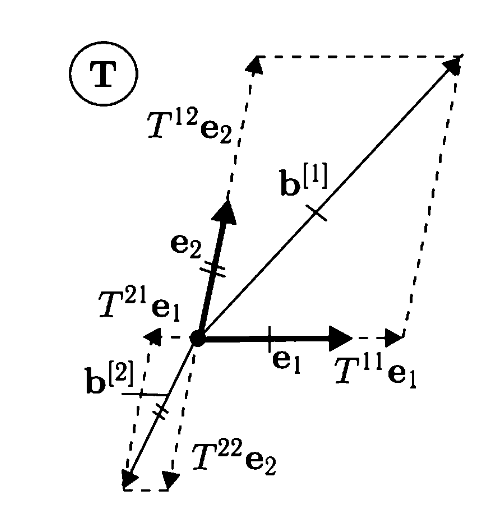
\includegraphics[width=\linewidth]{img/que3_1}
	\caption{Геометрическое изображение тензора $\mathbf{T}$в $E_{22}$}
	\end{subfigure}
	\hfill
	\begin{subfigure}{0.54\textwidth}
		\centering
	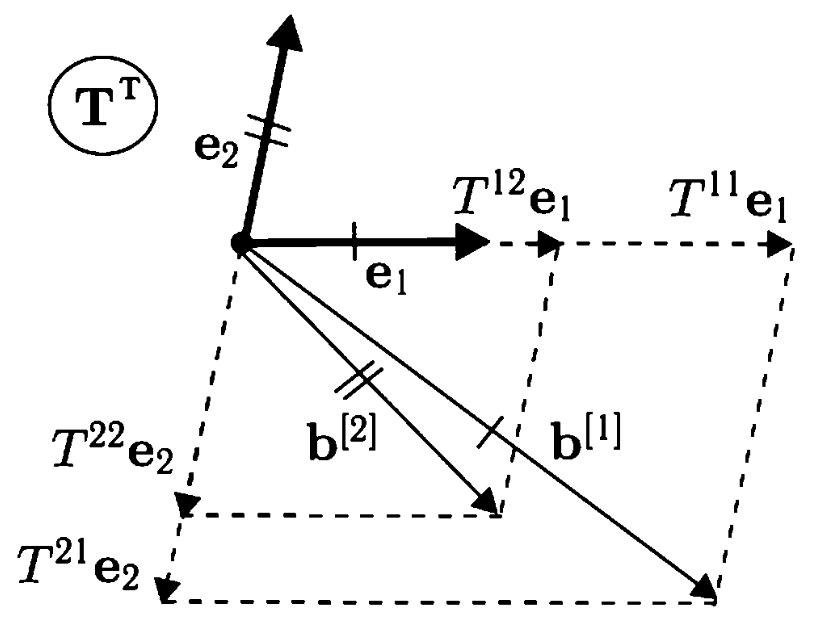
\includegraphics[width=\linewidth]{img/que3}
	\caption{Геометрическое изображение тензора $\mathbf{T}^T$, транспонированного к $\mathbf{T}$ в $E_{22}$}
	\end{subfigure}
	\hfill
	\caption{Иллюстрация к транспонированию тензоров}
	\label{fig:que3}
\end{figure}
\begin{remark}
	Для тензора $n$ порядка можно ввести $n!$ различных транспонированных тензора. (Количество возможных расстановок индексов.)
\end{remark}

\paragraph{Жонглирование индексами}
\textit{очевидно. жижки, камикадзе там.}
\paragraph{Скалярное умножение тензоров в евклидовых пространствах}
Умножение тензора на тензор:
\begin{equation*}
	\mathbf{T}\cdot\cdot\mathbf{B}=T^{ij}g_{jk}B^{kl}g_{il}
\end{equation*}
\begin{equation*}
	\mathbf{T}\cdot\mathbf{B}=\left(T^{ij}\mathbf{e}_i\otimes\mathbf{e}_j\right)\left(B^{lm}\mathbf{e}_l\otimes\mathbf{e}_m\right)=T^{ij}B^{lm}g_{jl}\mathbf{e}_i\otimes\mathbf{e}_m
\end{equation*}
Умножение тензора на вектор (см. Рисунок \ref{fig:que32}):
\begin{align*}
	\mathbf{T}\cdot\mathbf{c}&=T^{ik}c_k\mathbf{e}_i,\, \text{см. Рисунок \ref{fig:que32_ten_vec}},\\
	\mathbf{C}\cdot\mathbf{T}&=c_kT^{kj}\mathbf{e}_j,\, \text{см. Рисунок \ref{fig:que32_vec_ten}}.\\
\end{align*}
\begin{figure}[H]
	\hfill
	\begin{subfigure}{0.48\textwidth}
		\centering
		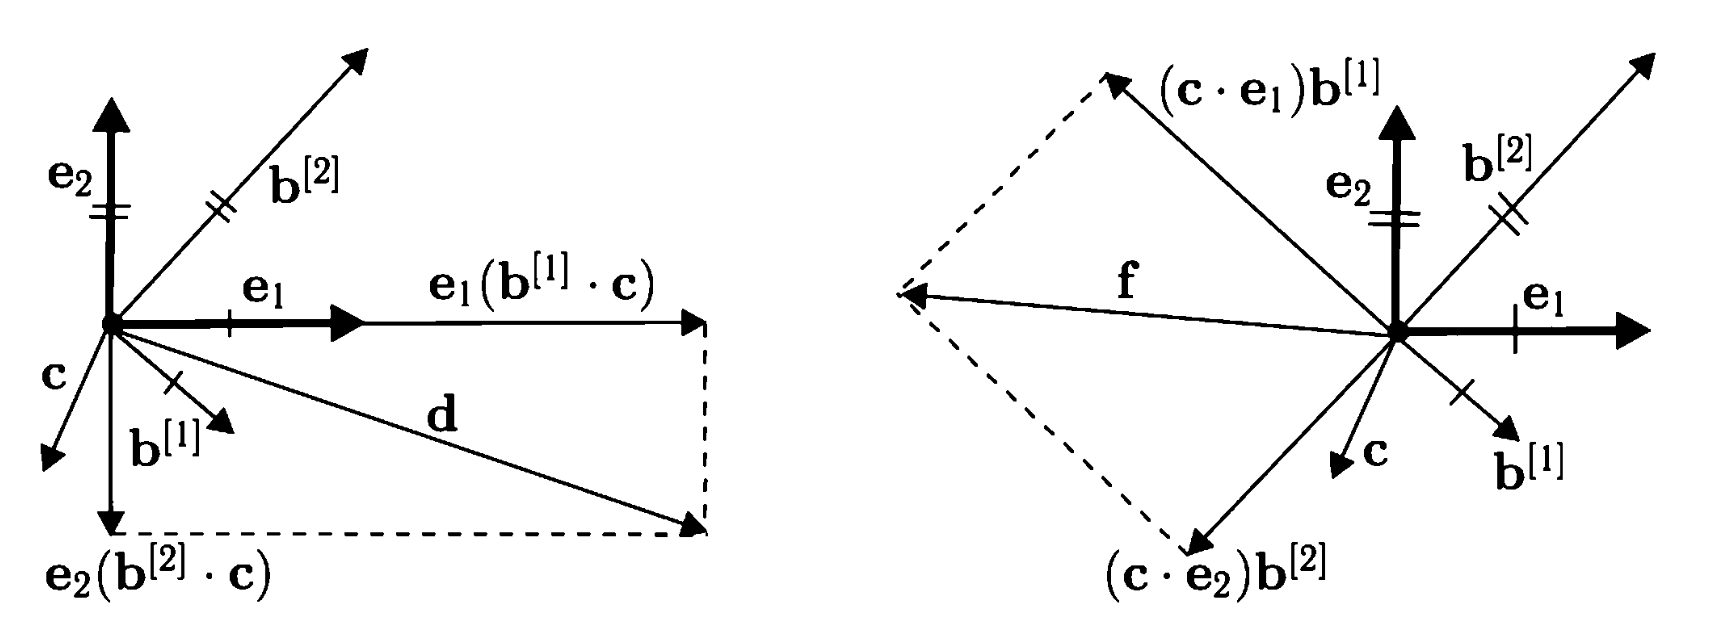
\includegraphics[width=0.7\linewidth,trim={0 0 12cm 0},clip]{img/que3_2}
		\subcaption{Геометрическое изображение скалярного произведения тензора на вектор справа: $\mathbf{T}\cdot\mathbf{c}$}
		\label{fig:que32_ten_vec}
	\end{subfigure}
	\hfill
	\begin{subfigure}{0.48\textwidth}
		\centering
		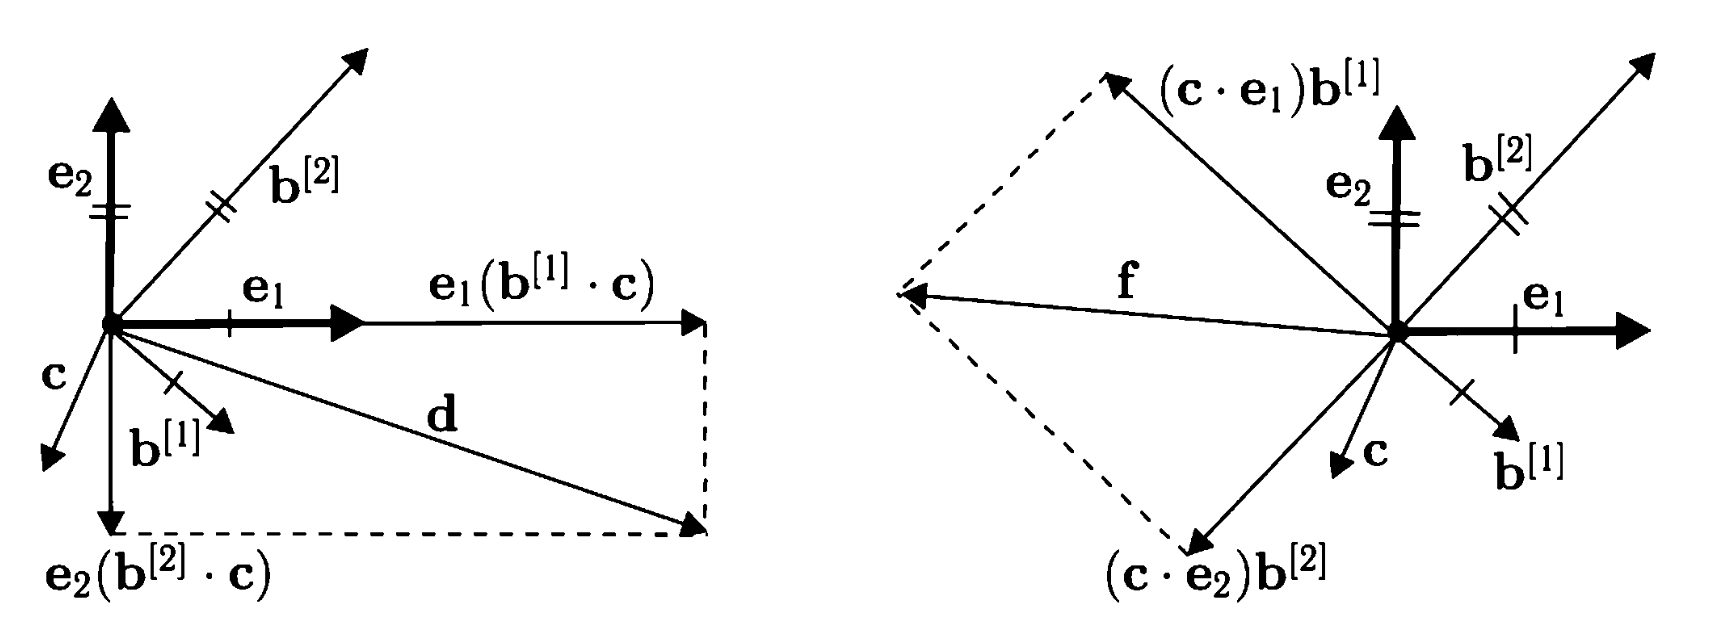
\includegraphics[width=0.7\linewidth,trim={11cm 0 0cm 0},clip]{img/que3_2}
		\subcaption{Геометрическое изображение скалярного произведения вектора на тензор слева: $\mathbf{C}\cdot\mathbf{T}$}
		\label{fig:que32_vec_ten}
	\end{subfigure}
	\hfill
	\caption{Скалярное умножение тензора на вектор}
	\label{fig:que32}
\end{figure}

\begin{utv}
	Двойное скалярное умножение тензора на базисные диады $\mathbf{e}_i\otimes\mathbf{e}_j$
\begin{equation*}
	\mathbf{T}\cdot\cdot\left(\mathbf{e}_i\otimes\mathbf{e}_j\right)=\mathbf{e}_i\cdot\mathbf{T}\cdot\mathbf{e}_j = T_{ij}
\end{equation*}
даёт компоненты этого тензора в диадном базисе $\mathbf{e}^i\otimes\mathbf{e}^j$.
\begin{proof}
	\begin{equation*}
		\mathbf{T}\cdot\cdot\left(\mathbf{e}_m\otimes\mathbf{e}_k\right)= T^{ij}\left(\mathbf{e}_i\otimes\mathbf{e}_j\right)\cdot\cdot\left(\mathbf{e}_m\otimes\mathbf{e}_k\right)=T^{ij}g_{jm}g_{ik}=T_{km}
	\end{equation*}
	Аналогичный результат получается и при умножении слева на $\mathbf{e}_i$ и справа на $\mathbf{e}_j$:
	\begin{equation*}
		\mathbf{e}_i\cdot\mathbf{T}\cdot\mathbf{e}_j = \mathbf{e}_i\cdot\left(T^{mk}\mathbf{e}_m\otimes\mathbf{e}_k\right)\cdot\mathbf{e}_j=
		T^{mk}\left(\mathbf{e}_i\cdot\mathbf{e}_m\right)\otimes\left(\mathbf{e}_k\cdot\mathbf{e}_j\right)=
		T^{mk}g_{im}g_{kj}=T_{ij}.
	\end{equation*}
\end{proof}
\end{utv}
\begin{utv}[Свойства скалярного произведения]
	Для произвольных тензоров второго ранга $\mathbf{T},\mathbf{B},\mathbf{A}\in\mathcal{E}_n^{(2)}$ и вектора $\mathbf{a}\in\mathcal{E}_2$ имеют место следующие соотношения:
	\begin{itemize}
		\item $\mathbf{a}\cdot\mathbf{A}=\mathbf{A}^T\cdot\mathbf{a}$;
		\item $\left(\mathbf{A}\cdot\mathbf{B}\right)^T=\mathbf{B}^T\cdot\mathbf{A}^T$;
		\item $\left(\mathbf{A}\cdot\mathbf{T}\right)\cdot\cdot\mathbf{B}=\mathbf{A}\cdot\cdot\left(\mathbf{T}\cdot\mathbf{B}\right)=\mathbf{B}\cdot\mathbf{A}\cdot\cdot\mathbf{T}=\mathbf{T}\cdot\mathbf{B}\cdot\mathbf{A}$;
		\item $\underbrace{\mathbf{A}\cdot\dots\cdot\mathbf{A}}_{k}=\mathbf{A}^k$
	\end{itemize}
\end{utv}

\begin{definition}[Единичный тензор 2 ранга]
	См. Рисунок \ref{fig:que33}.
	\begin{equation*}
		\mathbf{E} = \mathbf{e}_i\otimes\mathbf{e}^i = g^{ij}\mathbf{e}_i\otimes\mathbf{e}_j
	\end{equation*}
	В виде классов эквивалентности:
	\begin{equation*}
		\mathbf{E}=\left[\mathbf{e}_k\mathbf{e}^k\right]=\left[\mathbf{e}_1\mathbf{e}^1\dots\mathbf{e}_n\mathbf{e}^n\right]
	\end{equation*}
\end{definition}
\begin{figure}[H]
	\centering
	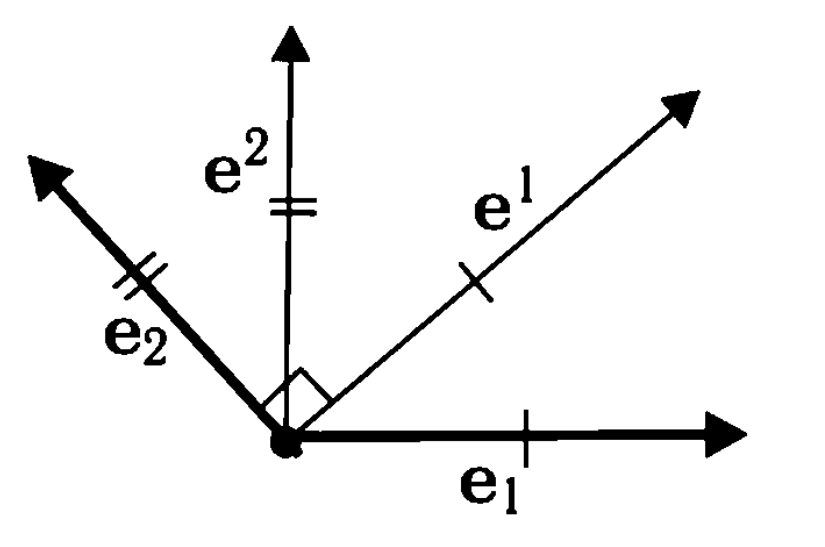
\includegraphics[width=0.4\linewidth]{img/que3_3}
	\caption{Геометрическое изображение единичного тензора в пространстве $\mathcal{E}_n^{(2)}\left(E_2\right)$}
	\label{fig:que33}
\end{figure}
